\documentclass[10pt,fleqn]{article}

\usepackage[english]{babel}
\usepackage[utf8x]{inputenc}
\usepackage{enumerate}
\usepackage{amsmath}
\usepackage{amssymb}
\usepackage{amsfonts} 
\usepackage{mathtools}
\usepackage{graphicx}
\usepackage{bm}
\usepackage[usenames,dvipsnames]{color}
\usepackage{todonotes}
\usepackage{dsfont}
\usepackage{hyperref}
\hypersetup{
    colorlinks,
    citecolor=black,
    filecolor=black,
    linkcolor=black,
    urlcolor=black
}
\usepackage{algorithm}
\usepackage{algorithmic}
\usepackage{appendix}
\usepackage{subcaption}
\usepackage{fancyvrb}
\usepackage{subfigure}
\usepackage{graphicx,xcolor}
\usepackage{pifont,mdframed}
\usepackage{tikz}
\usepackage{bm}
\usetikzlibrary{fit,positioning}


%
% Macros
%
\newcommand \cashort[1] { {\todo[color=yello]{#1 -- Cedric}} }
\newcommand \calong[1]  { { \todo[inline,color=yellow]{#1 -- Cedric} } }
\newcommand \gbshort[1] { {\todo[color=cyan!40]{#1 -- Guillaume}} }
\newcommand \gblong[1]  { { \todo[inline, color=cyan!40]{#1 -- Guillaume} } }
\newcommand \mgshort[1] { {\todo{#1 -- Mark}} }
\newcommand \mglong[1]  { { \todo[inline]{#1 -- Mark} } }
\newcommand \bfshort[1] { {\todo[color=green!40]{#1 -- Bryan}} }
\newcommand \bflong[1]  { { \todo[inline,color=green!40]{#1 -- Bryan} } }


% Adds a plus const to the end of a math expression
\def \pcst{+\text{const}}

% A fancy version for capital R
\def \Rcal{\mathcal{R}}

% A fancy version for r
\def \rcal{\mathbf{r}}

% Loss function / log likelihood as appropriate
\def \L{\mathcal{L}}

% KL divergence [Math Mode]
\newcommand{\kl}[2] {
	\text{KL}\left[#1||#2\right]
}

\newcommand \vecf[1] {
    \text{vec}\left(#1\right)
}

\newcommand \ent[1] {
    \text{H} \left[ #1 \right]
}

\newcommand \mut[2] {
    \text{I} \left[ #1 ; #2 \right]
}

\newcommand \dvi[2] {
    \text{D}_\text{VI} \left[ #1; #2 \right]
}

% Starts an expected value expresses [Math Mode]
\newcommand{\starte}[1] {%
	\mathbb{E}_{#1}\left[
}

% Ends an expected value expression [Math Mode]
\def \ende{\right]}

% Starts an varianc expresses [Math Mode]
\newcommand{\startv}[1] {%
	\mathbb{V}\text{ar}_{#1}\left[
}

% Ends an variance expression [Math Mode]
\def \endv{\right]}

%\newcommand \ex[2] {
%    \bigl\langle #1 \bigr\rangle_{#2}
%}
\newcommand \ex[2] {
    \mathbb{E}_{ { #2 } }\left[ #1 \right]
}
\newcommand \var[2] {
    \mathbb{V}ar_{ { #2 } }\left[ #1 \right]
}

\newcommand \halve[1] {
	\frac{#1}{2}
}

\newcommand \half {
    \halve{1}
}

\newcommand \tr { \text{tr} } 

\newcommand \T { ^\top } 

\newcommand \fixme[1] {
    {\color{red} FIXME: #1}
}

\newcommand \vv[1] { \bm #1 }

\newcommand{\mbeq}{\overset{!}{=}}

\newcommand \diag[1] { \text{diag} \left( {#1} \right) }
\newcommand \diagonal[1] { \text{diagonal} \left( {#1} \right) }

\newcommand \Ed {{ \vv{\xi}_d}}
\newcommand \Edj {{\xi_{dj}}}
\newcommand \Edk {{\xi_{dk}}}
\newcommand \AEdj {{\Lambda(\xi_{dj})}}
\newcommand \AEdk {{\Lambda(\xi_{dk})}}
\newcommand \AEd  {{ \bm{\Lambda}(\bm{\xi}_d) }}

\newcommand \Axi { { \Lambda_{\xi} } }
\newcommand \bxi { { \vv{b}_{\xi} } }
\newcommand \cxi { { c_{\xi} } }


\newcommand \wdoc      { { \vv{w}_d } }
\newcommand \wdt[0]  { { w_{dt} } }
\newcommand \wdn[0]  { { \vv{w}_{dn} } }
\newcommand \wdnt[0]  { { w_{dnt} } }
\newcommand \wdd[0]   { { \vv w_{d} } }
\newcommand \zd[0]   { { \vv z_{d} } }
\newcommand \zdn[0]  { { \vv{z}_{dn} } }
\newcommand \zdnk[0] { { z_{dnk} } }
\newcommand \zdk[0]  { { z_{dk} } }
\newcommand \thd[0]  { { \vv \theta_d } }
\newcommand \thdk[0] { { \theta_{dk} } }
\newcommand \thdj[0] { { \theta_{dj} } }
\newcommand \epow[1] { { e^{#1} } }
\newcommand \pkt     { { \phi_{kt}  } }
\newcommand \pk      { { \vv \phi_k } }
\newcommand \lmd     { { \vv \lambda_d } }
\newcommand \lmdk    { { \lambda_{dk} } }
\newcommand \xd      { { \vv x_d } }
\newcommand \atxd     { A ^\top \bm x_d}
\newcommand \axd     { A\bm x_d}
\newcommand \tsq      { { \tau^2 } }
\newcommand \ssq      { { \sigma^2 } }
\newcommand \tmsq     { { \tau^{-2} } }
\newcommand \asq      { { \alpha^2 } }
\newcommand \amsq     { { \alpha^{-2} } }
\newcommand \sgsq     { { \sigma^2 } }
\newcommand \xvec     { { \vv{x} } }
\newcommand \omk      { { \bm \omega _k } }
\newcommand \omkt     { { \omega_{kt} } }
\newcommand \oma     { { \Omega_A } }
\newcommand \gdn      { { \vv{\gamma}_{dn} } }
\newcommand \gdnk     { { \gamma_{dnk} } }
\newcommand \gdk      { { \gamma_{dk} } }
\newcommand \isigt   { { \Sigma^{-1}_{\bm \theta} } }




\newcommand \halfSig { \frac{1}{2\sigma^2} }

\newcommand \nor[2]   { \mathcal{N} \left( {#1}, {#2} \right) }
\newcommand \nord[3]   { \mathcal{N}_{#1} \left( {#2}, {#3} \right) }
\newcommand \mnor[3]  { \mathcal{N} \left(#1, #2, #3\right) }
\newcommand \norp[3]  { \mathcal{N} \left(#1; #2, #3\right) }
\newcommand \mnorp[4] { \mathcal{N} \left(#1; #2, #3, #4\right) }
\newcommand \mul[1]   { \mathcal{M} \left( {#1} \right) }
\newcommand \muln[2]  { \mathcal{M} \left( {#1},{#2} \right) }
\newcommand \dir[1]   { \mathcal{D} \left( {#1} \right) }
\newcommand \pois[1]  { \mathcal{P} \left( {#1} \right) }
\newcommand \gp[2]    { \mathcal{GP} \left( {#1}, #2 \right) }
\newcommand \dir[1]   { \mathcal{D} \left( {#1} \right) }
\newcommand \gam[2]   { \mathcal{G} \left( {#1}, {#2} \right) }
\newcommand \beta[1]  { \mathcal{B}eta \left( {#1}, {#2} \right) }

\newcommand \lne[1]  { { \ln \left( 1 + e^{ #1 } \right) } }
\newcommand \Tr[1]   { \tr \left(  {#1}  \right) }

\newcommand \roud  { \vv{\rho}_{d}  }
\newcommand \rodk { \rho_{dk} }

\newcommand \exA[1]  { \ex{#1}{q(A)} }
\newcommand \exV[1]  { \ex{#1}{q(V)} }
\newcommand \exT[1]  { \ex{#1}{q(\Theta)} }
\newcommand \extd[1] { \ex{#1}{q(\thd)} }
\newcommand \exTV[1] { \ex{#1}{q(\Theta)q(V)} }

\newcommand \Real[0]  { { \mathbb{R} } }
\newcommand \VReal[1] { { \mathbb{R}^{#1} } }
\newcommand \MReal[2] { { \mathbb{R}^{#1 \times #2} } }
\newcommand \Nat[0]  { { \mathbb{N} } }
\newcommand \VNat[1] { { \mathbb{N}^{#1} } }
\newcommand \MNat[2] { { \mathbb{N}^{#1 \times #2} } }

\newcommand \inv[1] { {#1}^{-1} }
\newcommand \invb[1] { \inv{\left( #1 \right)} }

\newcommand \cn { \textsuperscript{\texttt{[{\color{blue}Citation Needed}]}} }

\newcommand \const { { \text{c} } }

\providecommand \floor [1] { \left \lfloor #1 \right \rfloor }
\providecommand \ceil [1] { \left \lceil #1 \right \rceil }


\newcommand \vt[2] { { #1^{(#2)} } }

\newcommand \hashtag[1] { { \ttfamily \##1 } }

\newcommand \mvy  { \vv{m}_{\vv{y}} }
\newcommand \sigvy { { S_Y } }

\newcommand \mmy  { M_Y      }
\newcommand \md   { \vv{m}_d }
\newcommand \phin { \vv{\phi}_n }
\newcommand \isigma { { \inv{\Sigma} } }

\newcommand \sigv     { { \Sigma_V } }
\newcommand \isigv     { { \Sigma^{-1}_V } }

\newcommand \sigy { { \Sigma_Y } }
\newcommand \isigy { { \Sigma_{-1}_Y } }


\newcommand \omy  { { \Omega_Y } }
\newcommand \iomy { { \inv{\Omega_Y} } }

\newcommand \siga     { { \Sigma_A } }
\newcommand \isiga     { { \Sigma^{-1}_A } }
\newcommand \diagv { { \diag{\nu_1,\ldots,\nu_P} } }

\newcommand \ma { \vv{m}_a }
\newcommand \my { \vv{m}_y }

\newcommand \VoU { V \otimes U }

\newcommand \one { \mathbb{1} }
%\newcommand \one  {{  \mathds{1} }}

\newcommand \lse { \text{lse} }
%\newcommand \lse[0] { \mathrm{lse} }

% Conditional independence 
\def\ci{\perp\!\!\!\perp} % from Wikipedia



% ------ For the eval section

% Multinomial PDF [Math Mode]
% params: 1 - the variable
%         2 - the value
%         3 - the state indicator (e.g. k for a distro with K values)
%         4 - any additional subscript
\newcommand{\mpdf}[4] {
	\prod_{#3} {#1}_{{#4} {#3}} ^ {#2}
}

% Dirichlet PDF [Math Mode]
% params: 1 - the variable
%         2 - the hyper-parameter
%         3 - the state indicator (e.g. k for a distro with K values)
%         4 - any additional subscript
\newcommand{\dpdf}[4] {
	\frac{1}{B({#2})} \prod_{#3} {#1}_{{#4} {#3}} ^ {({#2}_{#3} - 1)}
}

% To simplify the sampling equations, this is indicates
% that the given value has had datapoint "m" stripped out
%
\newcommand{\lm}[1] {
	#1^{\setminus m}
}

\newcommand \model[0] {
    \mathcal{M}
}

\newcommand \perplexity[1] {
    \mathcal{P} \left( { #1 } \right)
}

\newcommand \WTrain {
    \mathcal{W}^{(t)}
}

\newcommand \WQuery {
    \mathcal{W}^{(q)}
}

\newcommand \oneover[1] {
    \frac{1}{ {#1} }
}

\newcommand \samp[1] {
    { #1 }^{(s)}
}

\newcommand \etd[0] {
    \vv{\eta}_d
}

\begin{document}



\newcommand \mnord[3] { { \mathcal{N}_{#1}\left({#2},{#3}\right) } }

\newcommand \const { { \text{c} } }

\providecommand \floor [1] { \left \lfloor #1 \right \rfloor }
\providecommand \ceil [1] { \left \lceil #1 \right \rceil }


\newcommand \vt[2] { { #1^{(#2)} } }

\newcommand \hashtag[1] { { \ttfamily \##1 } }

\newcommand \mvy  { \vv{m}_{\vv{y}} }
\newcommand \sigvy { { S_Y } }

\newcommand \mmy  { M_Y      }
\newcommand \md   { \vv{m}_d }
\newcommand \phin { \vv{\phi}_n }
\newcommand \isigma { { \inv{\Sigma} } }

\newcommand \sigv     { { \Sigma_V } }
\newcommand \isigv     { { \Sigma^{-1}_V } }

\newcommand \sigy { { \Sigma_Y } }
\newcommand \isigy { { \Sigma_{-1}_Y } }


\newcommand \omy  { { \Omega_Y } }
\newcommand \iomy { { \inv{\Omega_Y} } }

\newcommand \siga     { { \Sigma_A } }
\newcommand \isiga     { { \Sigma^{-1}_A } }
\newcommand \diagv { { \diag{\nu_1,\ldots,\nu_P} } }

\newcommand \ma { \vv{m}_a }
\newcommand \my { \vv{m}_y }

\newcommand \VoU { V \otimes U }

%\newcommand \one { \mathbb{1} }
\newcommand \one  {{  \mathds{1} }}

\newcommand \lse { \text{lse} }
%\newcommand \lse[0] { \mathrm{lse} }

% Conditional independence
\def\ci{\perp\!\!\!\perp} % from Wikipedia



% ------ For the eval section

% Multinomial PDF [Math Mode]
% params: 1 - the variable
%         2 - the value
%         3 - the state indicator (e.g. k for a distro with K values)
%         4 - any additional subscript
\newcommand{\mpdf}[4] {
	\prod_{#3} {#1}_{{#4} {#3}} ^ {#2}
}

% Dirichlet PDF [Math Mode]
% params: 1 - the variable
%         2 - the hyper-parameter
%         3 - the state indicator (e.g. k for a distro with K values)
%         4 - any additional subscript
\newcommand{\dpdf}[4] {
	\frac{1}{B({#2})} \prod_{#3} {#1}_{{#4} {#3}} ^ {({#2}_{#3} - 1)}
}

% To simplify the sampling equations, this is indicates
% that the given value has had datapoint "m" stripped out
%
\newcommand{\lm}[1] {
	#1^{\setminus m}
}

\newcommand \model[0] {
    \mathcal{M}
}

\newcommand \perplexity[1] {
    \mathcal{P} \left( { #1 } \right)
}

\newcommand \WTrain {
    \mathcal{W}^{(t)}
}

\newcommand \WQuery {
    \mathcal{W}^{(q)}
}

\newcommand \oneover[1] {
    \frac{1}{ {#1} }
}

\newcommand \samp[1] {
    { #1 }^{(s)}
}

\newcommand \etd[0] {
    \vv{\eta}_d
}

\newcommand \Ed {{ \vv{\xi}_d}}
\newcommand \Edj {{\xi_{dj}}}
\newcommand \Edk {{\xi_{dk}}}
\newcommand \AEdj {{\Lambda(\xi_{dj})}}
\newcommand \AEdk {{\Lambda(\xi_{dk})}}
\newcommand \AEd  {{ \bm{\Lambda}(\bm{\xi}_d) }}

\newcommand \Axi { { \Lambda_{\xi} } }
\newcommand \bxi { { \vv{b}_{\xi} } }
\newcommand \cxi { { c_{\xi} } }

\chapter{Jointly-Low Rank Admixture Models}
In the previous chapter, we investigated a correlated admixture model which employed low-rank projections of features in order to derive parsimonious model representations. A weakness of that model is that we increase the number of topics for a fixed dataset, there is a risk that the model becomes overparameterised once more: in particular the correlation matrix over topics may become singular.

In this chapter we provide an inference algorithm which enabled both low-rank feature \emph{and} topic covariance matrices. Standard application of the mechanics of variational inference would lead to an algorithm whose computational complexity was $O(P^3Q^3)$ where $P << F$ and $Q << K$ are the dimensions of our low-rank projections of the $F\times F$ covariance matrix over features and $K \times K$ covariance matrix over topics. We derive a novel algorithm instead whose computational complexity of $O(P^3 + Q^3)$, making inference in this model feasible.

\section{The Jointly Low-Rank Model}

The scenario is the same as in the previous chapter: features $\vv{x}_d$ with associate short texts $\wdoc$. We seek to assign topics to documents, so as to perform query expansion on them.

This is achieved by altering the manner in which we make predictions in the previous "YV" model to the following:

\begin{align}
Y \sim & \mnord{QP}{0}{\rho^2 I_P}{\alpha^2 I_Q} & A|Y \sim & \mnord{KF}{UYV\T}{\alpha^2 I_F}{\sigma^2 I_K} \\
\thd | A \sim & \nor{\axd}{\sigma^2 I_K}
\end{align}

Unfortunately, we can no longer obtain a matrix-variate marginal distribution over A, and so must use the multi-variate density to describe the marginal distribution.  

\begin{align}
\vecf{A} \sim \nor{\vv{0}}{\alpha^2 \sigma^2 I_{FK} + \rho^2 V\T V \otimes \tau^2 U\T U}
\end{align}

We refer to this as the reduced-covariance model.

\subsection{Variational Inference}
One approach to the reduced covariance model is to attempt to use matrix-variate posteriors with separate covariances -- $q(Y) \sim \mnord{QP}{M_Y}{R_Y}{S_Y}$, $q(A) \sim \mnord{KF}{M_A}{R_A}{S_A}$ --  despite the non-separability of the marginalized prior. However this immediately leads to a Sylvester equation, indicating that the covariance of the variational posterior is non-separable.

\begin{align}
\vecf{M_Y} = & \invb{\rho^{-2}\tau^{-2} I_{PQ} + \alpha^{-2}V V\T \otimes \sigma^{-2} U \T U}\vecf{\sigma^{-2}\alpha^{-2} U\T M_A V\T}
\end{align}

Collecting terms it's clear our approximate posterior over Y is a multivariate normal distribution over $\vecf{Y}$: $q(Y) = \nor{\vv{m}_y}{S_y}$. Using this we can recalculate the expectations of the affected terms in the free-energy

\begin{align}
\ex{p(Y)}{q} = & -\halve{PQ}\left(\ln 2\pi + \ln \rho^2 + \ln \tau^2\right) - \half \left(\rho^{-2}\tau^{-2} \vv{m}_y\T\vv{m}_y + \Tr{\rho^{-2}\tau^{-2} S_Y}\right) \\
\begin{split}
\ex{p(A|Y)}{q} = & -\halve{FK}\left(\ln 2\pi + \ln \rho^2 + \ln \tau^2\right) \\
 & -\half \Tr{\alpha^{-2}\sigma^{-2}(M_A - U M_Y V)(M_A - U M_Y V)\T} \\
 & -\half \Tr{S_Y \left(\alpha^{-2}V V\T \otimes \sigma^{-2}U \T U\right)} \\
 & -\half \Tr{\sigma^{-2}S_A\otimes \alpha^{-2}R_A}
 \label{eqn:free_enery_u_and_v}
\end{split}
\end{align}

Basic calculus gives us an update for Y

\begin{align}
S_y & = \invb{\rho^{-2} \alpha^{-2} I_{PQ} + V\T V \otimes U\T U}
&
\vv{m}_y & = S_y \vecf{U M_A V}
\end{align}

Unfortunately this requires inverting $S_y \in \mathbb{R}^{(P \times Q) \times (P \times Q)}$. This has a computational complexity of $O(P^3Q^3)$ which is not tractable. Therefore we develop the following method to reduce the computational complexity to $O(P^3 + Q^3)$ by analytically deriving the update for $Y$ from the eigen-decompositions of $U\T U$ and $V\T V$..

Recall that the eigen-decomposition of a matrix V is $U_V D_V U_V\T$ where $U$ is the matrix of V's eigen-vectors and $D$ a diagonal matrix of its eigen-values. The inverse is $\inv{V} = U_V \inv{D_V} U_V\T$, where the inverse of $D_V$, being diagonal, is trivially obtained. It has been shown in \cite{Stegle2011} that if $A = (a I + C \otimes B)$ then the eigen-decomposition is
\begin{align}
A = (a I + C \otimes B) = (U_C \otimes U_B)(\alpha I + D_C \otimes D_B)(U_C\T \otimes U_B\T)
\end{align}

We use this in our update for $\vv{m}_y = \vecf{M_Y}$. For brevity we use the change of notation $\vecf{U M_A V} = \vecf{T}$ and additionally denote the eigen-decompositions $U\T U = U_U D_U U_U\T$ and $V\T V = U_V D_V U_V\T$, given the revised update:

\begin{align}
\vecf{M_Y} = (U_V \otimes U_U)
  \invb{\alpha^{-2}\rho^{-2} I + S_V \otimes S_U}
  (U_V^\top \otimes U_U^\top) \vecf{T}
\end{align}

We can simplify this further. Letting $S = (\alpha^{-2}\rho^{-2} I + D_V \otimes D_U)$, we can define a second term $s$ according to

\begin{align}
S^{-1}(U_V^\top \otimes U_U^\top) \vecf{T} 
& =
(U_V^\top \otimes U_U^\top)S^{-1} \vecf{T} \\
& =
\vecf{U_U (\text{diag}(S^{-1})^{(Q)} .* T) U_V^\top} = s
\end{align}

where $.*$ denotes the Hadamard product, and we use the notation $A^{(p)}$ to denote the vec-transpose\cite{Minka2000a}. Further information on the vec-transpose operator is given in the appendix (section \ref{sec:vec-transpose} but not that $\vecf{A}^{(Q)} = \text{reshape}(A, rows=Q, cols=c)$.

Using the identity $\vecf{AXB} = (B\T \otimes A)\vecf{X}$ we can now re-write

\begin{align}
\vecf{M_Y} = (U_V \otimes U_U)s = \vecf{U_U^\top s^{(Q}) U_V}
\end{align}

Removing the vec operator from both sides and expanding terms we arrive at the final update for $Y$

\begin{align}
Y = U_U^\top (\diag{\inv{S}}^{(Q)} .* (U_U U M_A V U_V^\top)) U_V
\end{align}

\subsubsection{Inferring U and V}
The inference of U and V requires being able, in both cases, to differentiate the term

\begin{align}
\Tr{(V\T V \otimes U\T U)S_y} \label{eqn:kro-deriv-input}
\end{align}
which appears in the expectation of $\ex{\ln p(A)}{q}$.

As described in \cite{Minka2000a} taking derivates of Kronecker products involves the introduction of a \emph{commutation matrix} $T_{QP}$, a square, orthogonal, permutation matrix defined by the property that $T_{QP} \vecf{X} = \vecf{X\T}$. The derivatives of \eqref{eqn:kro-deriv-input} are (with apologies for the abuse of notation):

\begin{align}
\frac{d}{dU} \Tr{(V\T V \otimes U\T U)S_y} 
& = \left( \vt{(T_{QP} S_y)}{P} \right)\T (I_{PQ} \otimes V\T V)\vt{T_{QP}}{P}
\\
\frac{d}{dV} \Tr{(V\T V \otimes U\T U)S_y} 
& = \left(\vt{S_y}{Q}\right)\T (I_{PQ} \otimes U\T U) \vt{I_{PQ}}{Q}
\end{align}
The full derivation of these two results is given in the appendix, section \ref{sec:trace-kro-calculus}


\subsubsection{Inferring Document Level Topics}
Taking the derivates of the free-energy and setting to zero provides the following update for the distribution of topics for document $d$

\begin{align}
\md = & \invb{\sigma^{-2}I_K + N_d \Axi} \left(\sigma^{-2} M_A \xd  + N_d \bxi + Z^{(d)}\vv{w}_d \right )
\end{align}

As in the Low+Full model, this ostensibly involves a matrix inverse for every document, however by expanding terms and employing the Sherman-Morrison identity we can actually obtain the inverse analytically.

\begin{align}
\invb{\sigma^{-2}I_K + N_d \Axi}
& = \invb{(\sigma^{-2} + \halve{N_d})I_K + \frac{N_d}{2K + 2} \mathbf{1} \mathbf{1}\T} \\
& = \invb{a_d I_K + b_d \mathbf{1}\mathbf{1}\T} \\
& = \inv{a_d} I_K - \frac{{a_d}^{-2}b_d }{1 + \inv{b_d}K}\mathbf{1}\mathbf{1}\T
\end{align}

This provides an extremely efficient inference scheme. The full set of updates is given in algorithm \ref{alg:uyv}.

\newcommand \mvy  { \vv{m}_{\vv{y}} }
\newcommand \sigvy { { S_Y } }

\newcommand \mmy  { M_Y      }
\newcommand \omy  { \Omega_Y }
\newcommand \sigy { \Sigma_Y }

\subsection*{Matrix Calculus for Kronecker Products}
Solving for $U$ and $V$ requires the use of the vec-transpose \emph{operator} introduced in \cite{Wandell1992} and the \emph {communtation matrix} introduced in \cite{Magnus1988}. These are described here.

The vec-transpose of an $m \times n$ matrix $X$, denoted by $\vt{X}{p}$ is composed of $n$ submatrices stacked atop one another, where each $p \times ^m/_p$ sub-matrix is generated by a fortran-order reshaping of each column of X. The matrices are generated from top to bottom from the columns of X read from left to right. It generalizes both the transpose and $\vecf{\cdot}$ operations, as $\vt{X}{1} = X\T$ and $\vt{X}{\text{rows}(X)} = \vecf{X}$.

For an $m \times n$ matrix X, the commutation matrix is the square permutation matrix $T_{mn} \in \{0,1\}^{(m \times n) \times (m \times n)}$ that transforms $\vecf{X}$ into $\vecf{X\T}$ such that:
\begin{equation}
T_{mn} \vecf{X} = \vecf{X\T}
\end{equation}

With these we can define the following identities for the differentiation of terms in both sides of a Kronecker product. For the purpose of these identities only let $A \in \MReal{a}{nl}$, $X \in \MReal{m}{n}$ and $Y \in \MReal{k}{l}$ and thereby define

\begin{align}
\begin{split}
\frac{d}{dX} \Tr{A\T(X\T X \otimes Y\T Y)} & = 2X \left(\vt{A}{l}\right)\T (I_{nl} \otimes Y\T Y) \vt{I_nl}{l} \label{eqn:lhs_kro_derivative_symm}
\end{split} \\
\begin{split}
\frac{d}{dY} \Tr{A\T(X\T X \otimes Y\T Y)} & = 2 Y \left(\vt{(T_{ln} A)}{n}\right)\T (I_{nl} \otimes X\T X ) \vt{\left( T_{ln} \right)}{n} \label{eqn:rhs_kro_derivative_B_is_ident}
\end{split}
\end{align}

The vec-transpose operator and the commutation matrix and their applications to calculus are explained in more detail in \cite{Minka2000a}. The appendix provides a summary of the key points, and the derivations of \eqref{eqn:lhs_kro_derivative_symm} and \eqref{eqn:rhs_kro_derivative_B_is_ident}.

\subsection*{Derivation of the updates for U and V}

Starting first with V, we can use \eqref{eqn:lhs_kro_derivative_symm} to take the derivative of \eqref{eqn:free_enery_u_and_v} and so derive the following solution

\begin{equation}
V = \invb{\mmy\T U\T U \mmy + \left(\vt{S_Y}{Q}\right)\T (I_{PQ} \otimes U\T U) \vt{I_{PQ}}{Q} } \sigma^{-2} M_A \T U \mmy
\end{equation}

Next, for U, we employ \eqref{eqn:rhs_kro_derivative_B_is_ident} which provides the solution:
\begin{equation}
U = \invb{\mmy V\T V \mmy\T + \left( \vt{(T_{QP} S_Y)}{P} \right)\T (I_{PQ} \otimes V\T V)\vt{T_{QP}}{P}} M_A V \mmy\T
\end{equation}

Standard matrix calculus provide solutions for $\vv{m}_y $ and $S_Y$
\begin{align}
S_Y = & \invb{I_{mn} + V\T V \otimes U\T U}
& \vv{m}_y = & S_Y \vecf{U\T M_A V}
\end{align}


\begin{algorithm}
\caption{Representing $A=UYV$}
\label{alg:uyv}
$\text{ }$\\
{\bf E-Step}
    \begin{align*}
        & S_y = \invb{I_{mn} + V\T V \otimes U\T U} \quad &
Y & = U_U^\top (\diag{\inv{S}}^{(Q)} .* (U_U U M_A V U_V^\top)) U_V \\
        & &
        S & = (\alpha^{-2}\rho^{-2} I + D_V \otimes D_U) \\
        & S_A = \sigma^2 I_K \quad R_A = \invb{\alpha^{-2} I_F + \sigma^{-2} X\T X} 
        & M_A & = \left(\alpha^{-2} YV + \sigma^{-2} \sum_d \md \xd\T\right)R_A
    \end{align*}
    \begin{align*}
         \Vd = & \invb{\sigma^{-2}I_K + N_d \Axi}\\
         \md = & \invb{\sigma^{-2}I_K + N_d \Axi} \left(\sigma^{-2} M_A \xd  + N_d \bxi + Z^{(d)}\vv{w}_d \right )\\
        \gamma_{dvk} \propto & \beta_{kv} e^{m_{dk}} 
\end{align*}
{\bf M-Step}
\begin{align*}
    U = & \invb{\mmy V\T V \mmy\T + \left( \vt{(T_{QP} S_Y)}{P} \right)\T (I_{PQ} \otimes V\T V)\vt{T_{QP}}{P}} M_A V \mmy\T \\
    V = & \invb{\mmy\T U\T U \mmy + \left(\vt{S_Y}{Q}\right)\T (I_{PQ} \otimes U\T U) \vt{I_{PQ}}{Q} } M_A \T U \mmy \\
    \beta_{kv} \propto & \sum_d z_{dvk} w_{dv} 
\end{align*}
{\bf Bohning Bound M-Step}
    \begin{align*}
        \Axi & = \half \left(I_K - \mathbf{1}_K\mathbf{1}_K\T / K  \right) \\
        \bxi & = \Axi \vv{m}_d  - \sigma{\vv{m}_d}
    \end{align*}
\ref{alg:yv}
\end{algorithm}



\section{Experiments}
\begin{figure}
  \centering
    \hspace*{-1.5cm}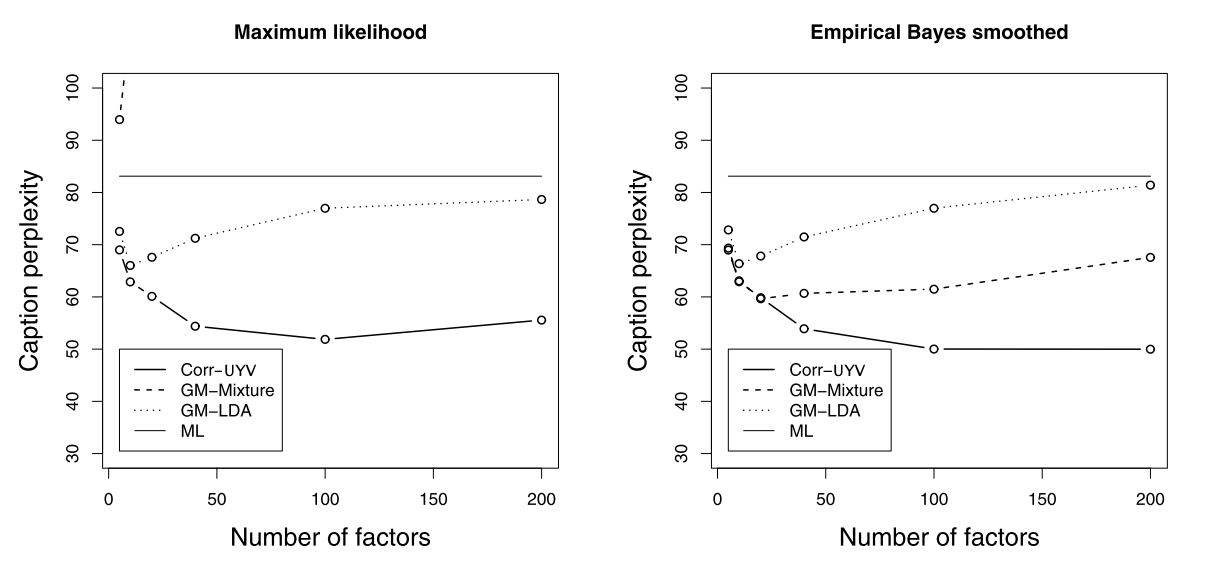
\includegraphics[height=0.25\textheight]{plots/figs/Fig5.png}
  \caption{Comparison between our model (``Corr-UYV") and other commonly used models}
  \label{fig:uyv-fig}
\end{figure}

In this section, we present an evaluation of all three mod-
els on 7000 images and captions from the Corel database. We held out 25\% of the data for testing purposes and used the remaining 75\% to estimate parameters. Each image is segmented into 6-10 regions and is associated with 2-4 caption words. The vocabulary contains 168 unique terms. We used the InceptionV3 neural network to extract features from the image in the dataset.

Our baseline was the GM-LDA model\cite{Blei2003} which uses a link-function to infer topic-strengths given simple LDA assignments.

\subsection{Test set likelihood }
To evaluate how well a model fits the data, we computed
the per-image average negative log likelihood of the test set on all three models for various values of K. A model which better fits the data will assign a higher likelihood to the test set (i.e., lower numbers are better in negative likelihood). Figure 5 illustrates the results. As expected, GM-LDA provides a much better fit than GM-Mixture.Further-more, Corr-LDA provides as good a fit as GM-LDA.This is somewhat surprising since GM-LDA is a less constrained model. However, both models have the same number of parameters; their similar performance indicates that, on aver- age, the number of hidden factors used to model a particular image is adequate to model its caption.

\subsection{Automatic annotation}
Given a segmented image without its caption, we can use
the mixture models described in Section 3 to compute a
distribution over words conditioned on the image, p(w| r). This distribution reflects a prediction of the missing caption words for that image.

To measure the annotation quality of the models, we com-
puted the perplexity of the given captions under $p(w| x)$ for each image in the test set. Perplexity,


Figure \ref{fig:uyv-fig} (Left) shows the perplexity of the held-out captions under the maximum likelihood estimates of each model for different values of K. We see that overfitting is a serious problem in the GM-Mixture model, and its perplexity immediately grows off the graph (e.g., when K = 200, the perplexity is 2922). Note that in related work, many of the models considered are variants of GM-Mixture and rely heavily on an ad-hoc smoothing procedure to correct for overfitting. Figure \ref{fig:uyv-fig} (Right) illustrates the caption perplexity under
the smoothed estimates of each model using the empirical Bayes procedure. The overfitting of GM- Mixture has been corrected. Once smoothed, it performs better than GM-LDA despite the GM-LDA model’s superior performance in joint likelihood. We found that GM-LDA does not provide good conditional distributions for two reasons. First, it is ``over-smoothed." Computing $p(w| x)$ requires integrating a dif- fuse posterior (due to the small number of regions) over all the factor dimensions. Thus, the factors to which each region is associated are essentially washed out and, as K gets large, the model’s performance approaches the performance of the simple maximum likelihood estimate of the caption words.

\begin{figure}
  \centering
    \hspace*{-1.5cm}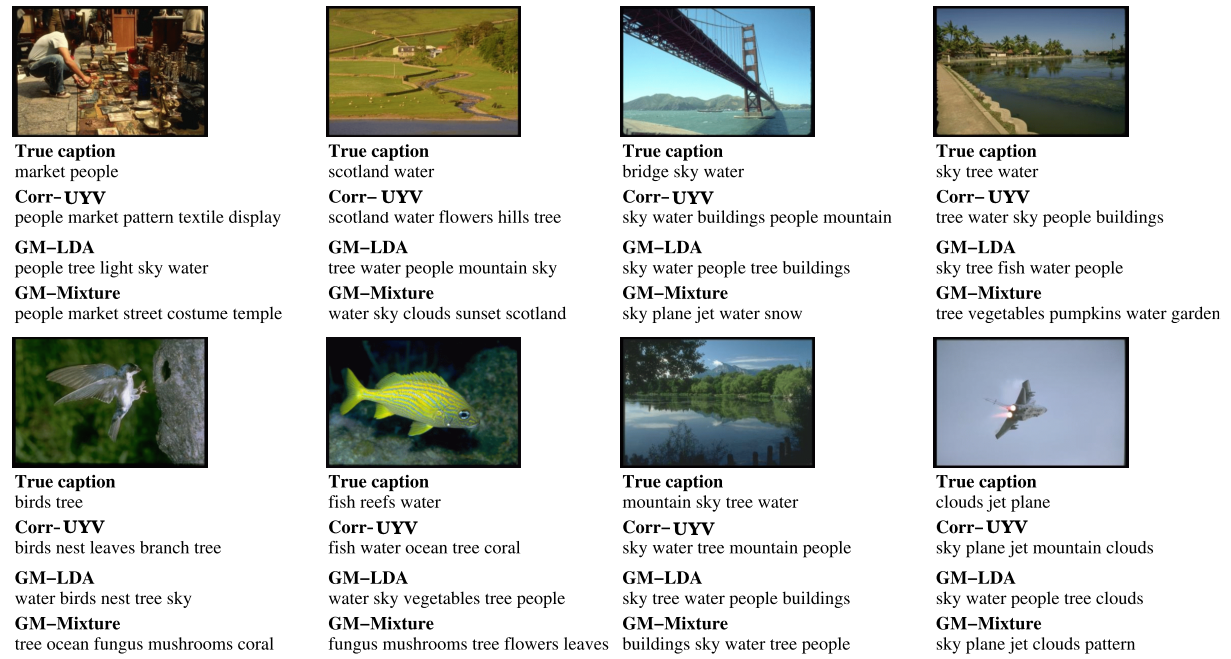
\includegraphics[height=0.40\textheight]{plots/figs/Fig2.png}
  \caption{Sample annotations for various images}
  \label{fig:uyv-fig}
\end{figure}

Second, GM-LDA easily allows caption words to be generated by factors that did not contribute to generating the image regions (e.g., when K = 200, 54\% of the caption words in the test set are assigned to factors that do not appear in their corresponding images). With this freedom, the estimated conditional Gaussian parameters do not necessarily reflect regions that are correctly annotated by the corresponding conditional multinomial parameters. While it better models the joint distribution of words and regions, it fails to model the relationship between them. Most notably, Corr-LDA finds much better predictive
distributions of words than either GM-LDA or GM-Mixture. It provides as flexible a joint distribution as GM-LDA but guarantees that the latent factors in the conditional Gaussian (for image regions) correspond with the latent factors in the conditional multinomial (for caption words). Furthermore, by allowing caption words to be allocated to different factors, the Corr-LDA model achieves superior performance to the GM-Mixture which is constrained to associating the entire image/caption to a single factor. Thus, with Corr-LDA, we can achieve a competitive fit of the joint distribution and find superior conditional distributions of words given images

Figure \ref{fig:uyv-images} shows ten sample annotations—the top five words
from $p(w|x)$ computed by each of the three models for K = 200. These examples illustrate the limitations and
power of the probabilistic models described in Chapter 1 when used for a practical discriminative task

The GM-LDA model, as shown quantitatively in the previous section, gives the least impressive performance of the three. First, we see washing out effect described above by the fact that many of the most common words in the corpus — words like “water” and “sky” — occur in the predicted captions for all of the pictures. Second, the predicted caption rarely predicts the object or objects that are in the picture. For example, it misses “jet” in the picture captioned clouds, jet, plane, a word that both other models predict with high accuracy. The GM-Mixture model performs better than GM-LDA, but we can see how this model relies on the average image features and fails to predict words for regions that may not generally occur in other similar images. For example, it omits “tree” from the picture captioned scotland, water since the trees are only a small part on the left side of the frame. Furthermore, the GM-Mixture predicts completely incorrect words if the average features do not easily correspond to a common theme. For example, the background of fish, reefs, water is not the usual blue and GM-Mixture predicts words like “fungus”, “tree”, and “flowers.” Finally, as reflected by the term perplexity results above,
the Corr-LDA model gives the best performance and correctly labels most of the example pictures. Unlike the GM- Mixture model, it can assign each region to a different cluster and the final distribution over words reflects the ensemble of clusters which were assigned to the image regions. Thus, the Corr-LDA model finds the trees in the picture labeled scotland, water and can correctly identify the fish, even without its usual blue background.

\section{Conclusion}
We have presented a novel method, with fast, efficient inference, for incorporating features into topics. Our method avoids the issues of singular matrices that occur when estimating large covariance parameters from few parameters. Our method also, it should be said, provides the basis for a fast, efficient, two-dimensional PCA algorithm.

A disadvantage of our method is the need to determine the latent dimensions in advance. In practice, in our results, this was obtained by grid-search, but this is highly time-consuming.

Nevertheless, our model provides a useful means for augmenting existing image captioning schemes.

\bibliographystyle{plain}
\bibliography{/Users/bryanfeeney/Documents/library.bib}

\end{document}
